\documentclass[tikz,border=10pt]{standalone}
\usepackage{tikz}
\usepackage{fontawesome5}
\usetikzlibrary{shapes.geometric,arrows.meta,positioning,fit,backgrounds,calc}

\begin{document}
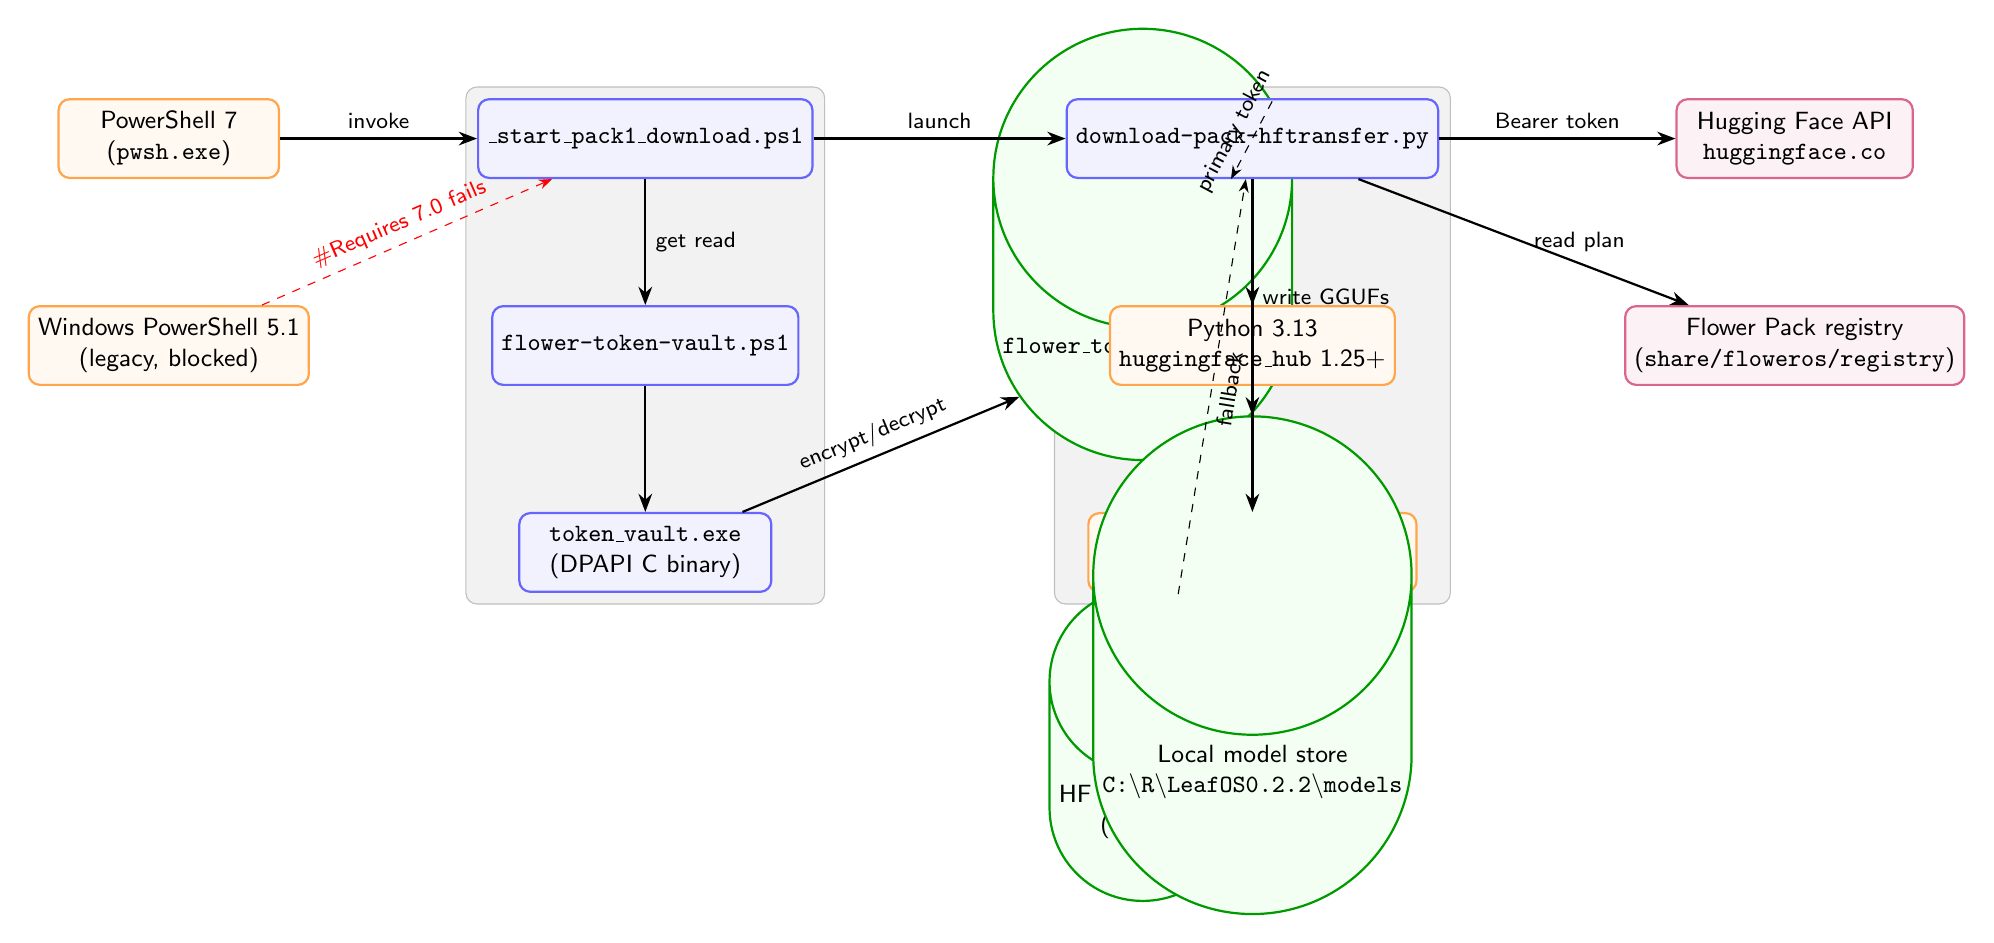
\begin{tikzpicture}[
	font=\sffamily\small,
	node distance=1.6cm and 2.2cm,
	>=Stealth,
	box/.style={rectangle, rounded corners, draw=blue!60, fill=blue!5, minimum width=3.2cm, minimum height=1cm, align=center, thick},
	exec/.style={rectangle, rounded corners, draw=orange!70, fill=orange!5, minimum width=2.8cm, minimum height=1cm, align=center, thick},
	data/.style={cylinder, shape border rotate=90, draw=green!60!black, fill=green!5, minimum width=2cm, minimum height=1cm, align=center, thick},
	ext/.style={rectangle, rounded corners, draw=purple!60, fill=purple!5, minimum width=3cm, minimum height=1cm, align=center, thick},
	label/.style={rectangle, draw=gray!50, fill=gray!10, rounded corners, inner sep=4pt, font=\bfseries\small}
]

% --- Top: user entry points ---
\node[exec] (pwsh7) {PowerShell 7\\(\texttt{pwsh.exe})};
\node[exec, below=of pwsh7] (wp51) {Windows PowerShell 5.1\\(legacy, blocked)};

% --- Middle: orchestration ---
\node[box, right=2.5cm of pwsh7] (start) {\texttt{\_start\_pack1\_download.ps1}};
\node[box, below=of start] (vaultps) {\texttt{flower-token-vault.ps1}};
\node[box, below=of vaultps] (vaultc) {\texttt{token\_vault.exe}\\(DPAPI C binary)};

% --- Token/data stores ---
\node[data, right=2.5cm of vaultps] (vaultfile) {\texttt{flower\_token\_vault.dat}};
\node[data, below=of vaultfile] (cache) {HF cache token\\(\texttt{token})};

% --- Downloader core ---
\node[box, right=3.2cm of start] (downloader) {\texttt{download-pack-hftransfer.py}};
\node[exec, below=of downloader] (py313) {Python 3.13\\\texttt{huggingface\_hub} 1.25+};
\node[exec, below=of py313] (hftransfer) {Rust backend\\(\texttt{HF\_XET\_HIGH\_PERFORMANCE})};

% --- External sources ---
\node[ext, right=3cm of downloader] (hfapi) {Hugging Face API\\\texttt{huggingface.co}};
\node[ext, below=of hfapi] (registry) {Flower Pack registry\\(\texttt{share/floweros/registry})};

% --- Output ---
\node[data, below=3cm of downloader] (models) {Local model store\\\texttt{C:\textbackslash R\textbackslash LeafOS0.2.2\textbackslash models}};

% --- Edges ---
\draw[->, thick] (pwsh7) -- (start) node[midway,above,sloped] {\footnotesize invoke};
\draw[->, dashed, red] (wp51) -- (start) node[midway,above,sloped] {\footnotesize \#Requires 7.0 fails};
\draw[->, thick] (start) -- (vaultps) node[midway,right] {\footnotesize get read};
\draw[->, thick] (vaultps) -- (vaultc);
\draw[->, thick] (vaultc) -- (vaultfile) node[midway,above,sloped] {\footnotesize encrypt/decrypt};
\draw[->, thick] (start) -- (downloader) node[midway,above] {\footnotesize launch};
\draw[->, thick] (downloader) -- (py313);
\draw[->, thick] (py313) -- (hftransfer);
\draw[->, thick] (downloader) -- (registry) node[midway,right] {\footnotesize read plan};
\draw[->, thick] (downloader) -- (hfapi) node[midway,above] {\footnotesize Bearer token};
\draw[->, thick] (downloader) -- (models) node[midway,right] {\footnotesize write GGUFs};
\draw[->, dashed] (cache) -- (downloader) node[midway,below,sloped] {\footnotesize fallback};
\draw[->, dashed] (vaultfile) -- (downloader) node[midway,above,sloped] {\footnotesize primary token};

\begin{scope}[on background layer]
  \node[fit=(start)(vaultc),fill=blue!3,rounded corners,inner sep=10pt,label={[label]above left:Windows install layer}]{\hspace{1cm}};
  \node[fit=(downloader)(hftransfer),fill=orange!3,rounded corners,inner sep=12pt,label={[label]above right:Download engine}]{\hspace{1cm}};
\end{scope}

\end{tikzpicture}
\end{document}
